\documentclass{acm_proc_article-sp}
\usepackage{url}
\usepackage{graphicx}
\begin{document}
\title{Sheetmusic: Making music from spreadsheets}
\numberofauthors{1}
\author{
\alignauthor
Thomas Levine\\
       \affaddr{csv soundsystem}\\
       \email{\_@thomaslevine.com}
}
\date{6 March 2014}
\maketitle
\begin{abstract}
The spreadsheet provides an intuitive paradigm for the expression of musical
scores. Musical scores can be expressed as data tables, with each record
corresponding to a place in time and each column corresponding to a note
or instrument. Sheetmusic is a plugin for Gnumeric that provides music
sequencing spreadsheet functions. Tools like Sheetmusic provide intuitive
music composition interfaces for people who are used to data analysis software.
Moreover, they help us plot data with the sense of sound.
\end{abstract}
\keywords{music, spreadsheets, gastronomification, data analysis}
\section{Non-visual displays of quantitative information}
Data analyists often use visualization as a means for plotting data,
but there are other approaches!

\subsection{Data sonification}
Just as data can be expressed visually, data can also be expressed
in sound. As demonstration of this, Ferguson \& al. \cite{ferguson}
created auditory analogs for simple
visual plots, such as the dotplot and boxplot.

Visual plots are far more common than auditory plots. Why is this?
My hunch is that our technology for visual rendering is simply much
further advanced; printing technology has been around for centuries,
and writing has been around for millenia. With this history, we have
also developed advanced theory related to the visual plotting of data.
Audio recording is a comparably recent invention, and our theory around
auditory plotting is accordingly less developed.

In my view, we separate data sonification from data visualization
only because of technological constraints; there isn't a fundamental
difference between these two processes.

\subsection{Data-driven music videos}
\begin{figure*}
\centering
\includegraphics[width=\textwidth]{../sensory-data-experiences/fms.png}
\caption{Here is a frame from the FMS Symphony video. I unfortunately can't play the accompanying song in this paper.}
\label{fms}
\end{figure*}

Combining the visual and auditory senses, we can plot data in the form
of music videos. One example of this is the FMS Symphony (figure \ref{fms}).
In the FMS Symphony, each beat of music corresponds to a business day
during the period between 2005 and 2013, the pitch of one instrument
corresponds to the United States interest rate, the pitch of another
instrument corresponds to the distance to the United States debt ceiling,
and the activation of certain flourishes corresponds to changes in the
balance of the United States treasury. These data are also represented
visually, through the combination of an animated line plot and a
Chernoff face \cite{fms-about}.

\subsection{Food}
Why stop at just vision and hearing? We can plot data as food and use
all five senses. One example of this is Census Spices, a set of spices
that represent different neighborhoods based on demographics collected
by the United States Census \cite{censusspices}.

\section{Our tools for musical plotting}
We at csv soundsystem have been exploring multisensory
data plotting methods, including music videos and food.
In our production of data-driven music videos, we have recognized a need
for data analysis software and music software to be more strongly integrated.
We wanted a more seamless transition between modeling and music, and we
wanted it to be easier for data analysts to work with music. We have
developed tools like Sheetmusic to bridge this gap.

To use the language of the Grammar of Graphics, \cite{grammar}
we have abstract data and concrete plot elements,
and we define aesthetics that provide mappings
between the abstract data and the concrete elements.
The primitive plot elements that we use for music are things
like key, rhythm, pitch, and interval.

\subsection{Data tables}
We've found that the tabular representation of data aligns very well with
typical representations of music. Our data music tools work by mapping these
two concepts to each other.

We can think of data tables as collections of similar things, with the
same sorts of information being collected about each thing. In tidy data
tables \cite{tidydata} each row corresponds to an observation (a thing),
and each column corresponds to a variable. We add more rows to the table
as we observe more things, and we add more columns to the table as we
collect more information about each thing.

We can think of music as a composition of many different sounds over time,
with sounds coming from many different instruments. In musical scores
we represent time as movement from left to right, and we represent different
notes played at the same time by different dots on a staff,
The staff becomes wider as the song gets longer, (They are often spread
across multiple pages.) and we add more dots as we add more notes
(figure \ref{highlight}).

Rather than composing music as traditional sheet music,
we can use a table-editing program of our choice to compose
this sort of table. Our data music software simply adds
musical functions to table containers in various data analysis
tools.

\begin{figure*}
\centering
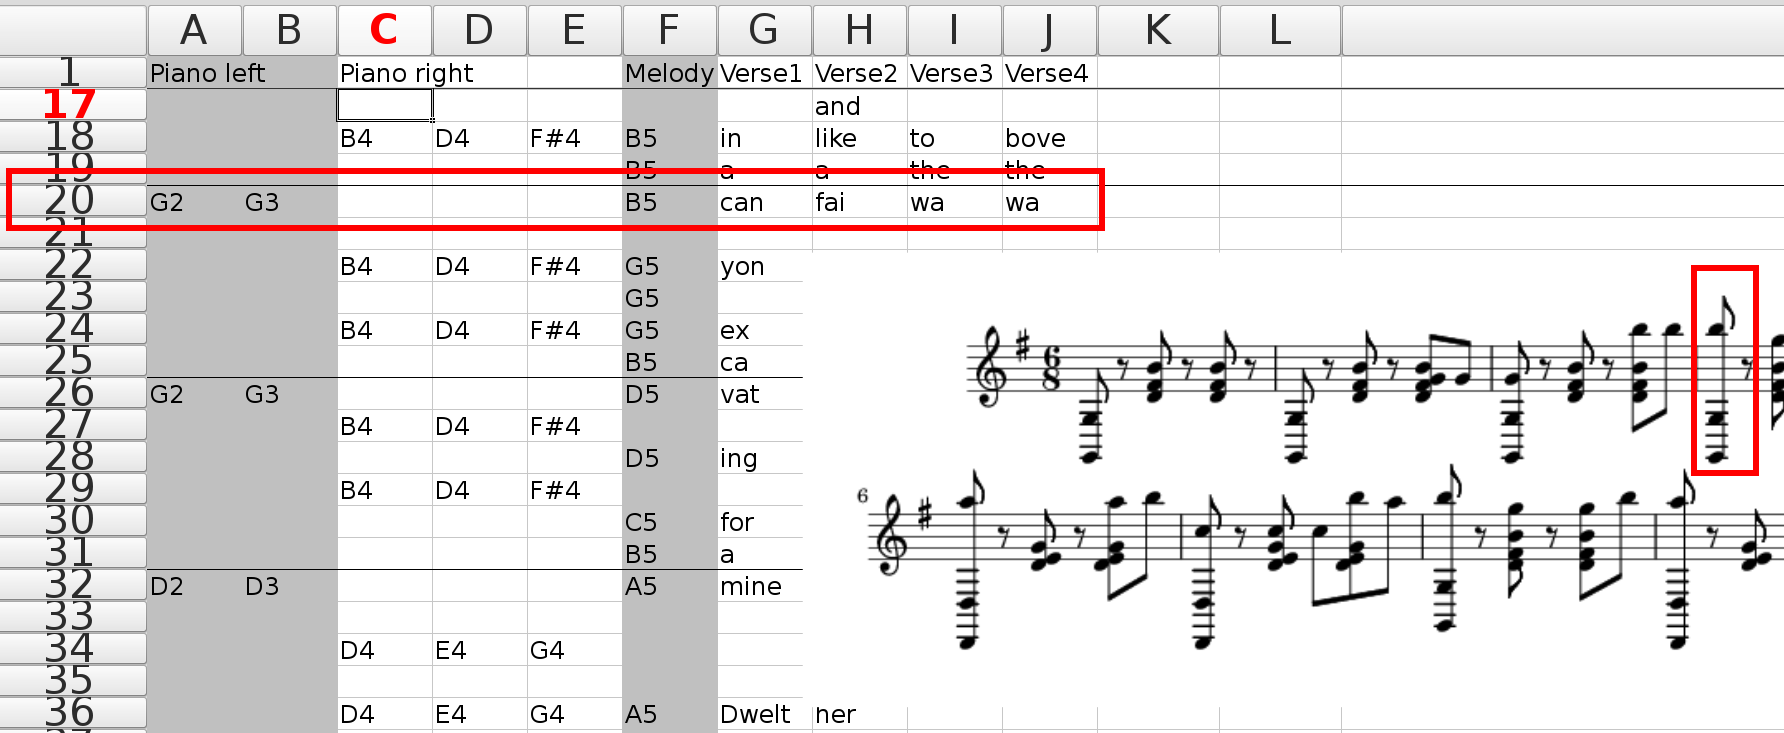
\includegraphics[width=\textwidth]{../sheetmusic/sheetmusic-side-by-side-highlighted-rowbeat.png}
\caption{A spreadsheet is displayed alongside some corresponding ordinary sheet music, with a corresponding row/beat highlighted.}
\label{highlight}
\end{figure*}


Sheetmusic is our offering for spreadsheets, but we
also have libraries for R data frames \cite{ddr} and Pandas
data frames \cite{ddpy}.

\section{How to use Sheetmusic}
Let's divide Sheetmusic's features into two groups. The first group
is spreadsheet functions for music synthesis---these are functions
like \texttt{CHORD\_PROGRESSION} that take spreadsheet cells or values
as input and return values to other spreadsheet cells. The second
group is functions for rendering the music to external devices,
including MIDI and sheetmusic.

\subsection{Organization of the spreadsheet}
Sheetmusic expects that the spreadsheet be organized as follows.
Each column corresponds
to a musical track, and different tracks can have different music instruments.
Row corresponds to a beat (of time).
Each cell contains the frequency of sound to be played, represented
in scientific notation (C4, D4, \&c.).

\subsection{Composing music}
The data analyst can use conventional spreadsheet approaches for
composing music. For example, the following function can be used
to produce a major scale in a spreadsheet column.

\begin{verbatim}=IONIAN_SCALE("A4")\end{verbatim}

Once you have a major scale in one column, you can easily make
chords with a spreadsheet functions like this.

\begin{verbatim}=MAJOR_THIRD_INTERVAL(B1)\end{verbatim}

If you put this in cell B1, A1 and B1 will form a major third interval.

\subsection{Rendering music}
\begin{figure}
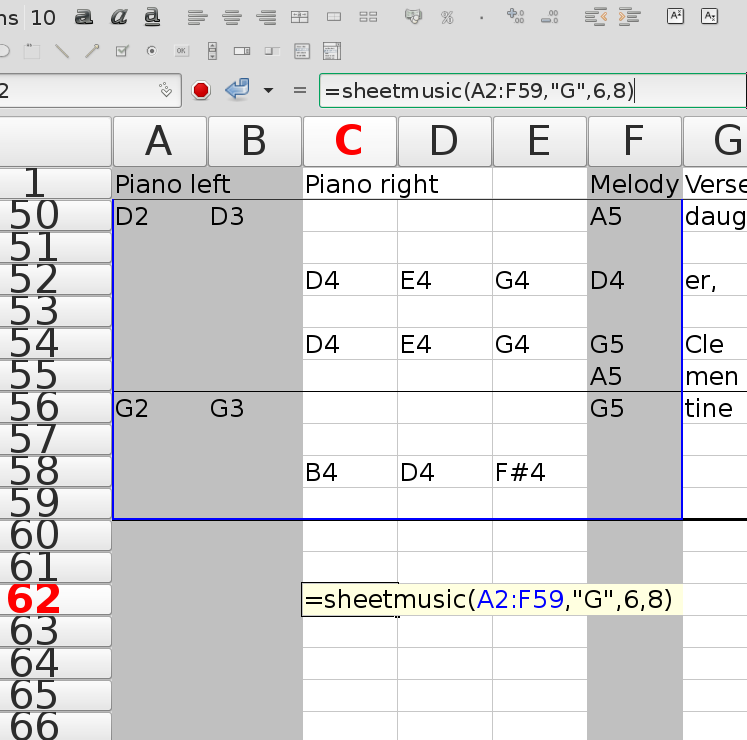
\includegraphics[width=\columnwidth]{../sheetmusic/sheetmusic-function-call.png}
\centering
\caption{Using Sheetmusic to render a spreadsheet as sheetmusic}
\end{figure}

Once we have composed our piece, we can select the appropriate cells,
specify the key and time signatures of the piece, and export it as
MIDI or sheetmusic.

It is possible, of course, to convert to any number of music formats,
just as we can convert spreadsheets to any number of data table formats.
Only MIDI and sheetmusic are implemented at present, but you can
indirectly convert to many formats by first saving as MIDI and then
converting from MIDI to your output format of choice.

\subsection{Musical plots}
I've discussed how we can use Sheetmusic for conventional music
composition. To use it as a plotting tool, we simply have to map
our abstract data to musical notes. Sheetmusic provides the
\texttt{FROMWHOLENUMBER} function to enable this. If we imagine an
infinitely wide piano with the C0 as the left-most note,
\texttt{FROMWHOLENUMBER} starts at C0 and walks $i$ keys to the right,
where $i$ is the argument passed to \texttt{FROMWHOLENUMBER}.

After using ordinary spreadsheet modeling functions to manipulate data,
a user may scale and round the data appropriately and then run
\texttt{FROMWHOLENUMBER} to convert them into notes.

\section{Relevance}
I hope that I've shown how data can be plotted in the form of music.
I would be remiss not to discuss the merits of this plotting method.

\subsection{Easier composition of music}
When we plot data as music, we effectively let data compose music for us.
We still have to choose datasets that will produce interesting music and
map the data to the music appropriately, but the randomness of the data
can provide the various subtleties of music that we would otherwise have
to design ourselves.

\subsection{Data literacy}
When we start using data analysis software for other things,
we blur the line between data analysis and other things.
Data analysis seems very magical to many people. When we represent
data as familiar things like music, people seem to be a bit less
scared of data analysis.

\subsection{Expressing high-dimensional datasets}
The use of multiple senses may also allow for the expression of
high-dimensional datasets. Tufte advocates for the production of
visuals that express the multivariate nature of the world.\cite{tufte}
I think that the use of multiple senses has the potential to
facilitate the expression of more easily express many variables at
once, and this may aid in the identification of high-dimensional
relationships.

\bibliographystyle{abbrv}
\bibliography{spreadsheets}
\balancecolumns
\end{document}
